\subsection{Underlying Event estimation}
\label{sec:UEsubtraction}
In this section, we describe how we estimate and subtract the ``underlying event'' (UE). The UE is defined as the particles not associated with the hard-scattering of the collision\footnote{In Ref.~\cite{ALICE:2011ac}, the UE is defined as ``the sum of all the processes that build up the final hadronic state in a collisions excluding the hardest leading order partonic interaction. This includes fragmentation of beam remnants, multi-parton interactions and initial and final-state radiation associated with each interaction."}. We subtract the UE from the measured transverse momentum of jets and in the photon isolation (described in Section~\ref{sec:isolation}). 
Technically, the discrimination between the soft component from the hard component of an event is performed using the \textsc{Fastjet} jet area/median method~\cite{Cacciari:2009dp}, which uses the median of the distribution of transverse momentum densities of all jets in an event. We use one of the standard jet areas definition implemented in \textsc{FastJet} called Voronoi area~\footnote{The method used is the following fastjet::VoronoiAreaSpec \url{http://www.fastjet.fr/repo/doxygen-2.4.5/classfastjet_1_1VoronoiAreaSpec.html} }.

The estimation of the UE density uses jets $J'$ reconstructed by the
$k_{\mathrm{T}}$-algorithm\footnote{In contrast to the anti-$k_{\mathrm{T}}$ algorithm, the $k_{\mathrm{T}}$ algorithm clusters the softest particles first, and thus is more sensitive to the details of the distribution of softer objects and better suited for an investigation of the underlying event.} with distance parameter $R=0.3$. The estimated UE
density is defined as:
\begin{equation}
  \rho = \mathrm{med} \left\{ \frac{\sum_{i\in J'_k}
    p_{T,i}}{\sum_{i\in J'_k} A_i} \right\}
\end{equation}
where $p_{T,i}$ is the transverse momentum, and $A_i$ the Voronoi area
of the particle $i$ within the jet reconstructed for UE estimation
purpose $J'_k$. Following standard practice, the two leading jets are not considered in this observable, to limit the contribution from the hard component of the interaction. 

The choice of the median is motivated by its robustness against outliers, which includes jets originated by hard interactions. The observable
thus isolates UE  by assuming that most of the event is either empty or dominated by soft contributions and that the hard component of the interaction is well contained within the leading jets~\citep{Cacciari:2009dp}. 

Figure~\ref{fig:Rho} shows the median charged-particle density, $\rho$, distribution obtained in pp and p-Pb data in minimum bias events and in events that pass the selection in Section~\ref{sec:eventselection} and thus have a high-$\pt$ cluster. The distribution in minimum-bias events decreases approximately exponentially. The distribution in photon-triggered events is different and follows sort of an asymmetric Gaussian distribution that peaks at approximately {1.0 \GeVc} and {2.5 \GeVc} for pp and \pPb~collisions, respectively. 
\begin{figure}
\center
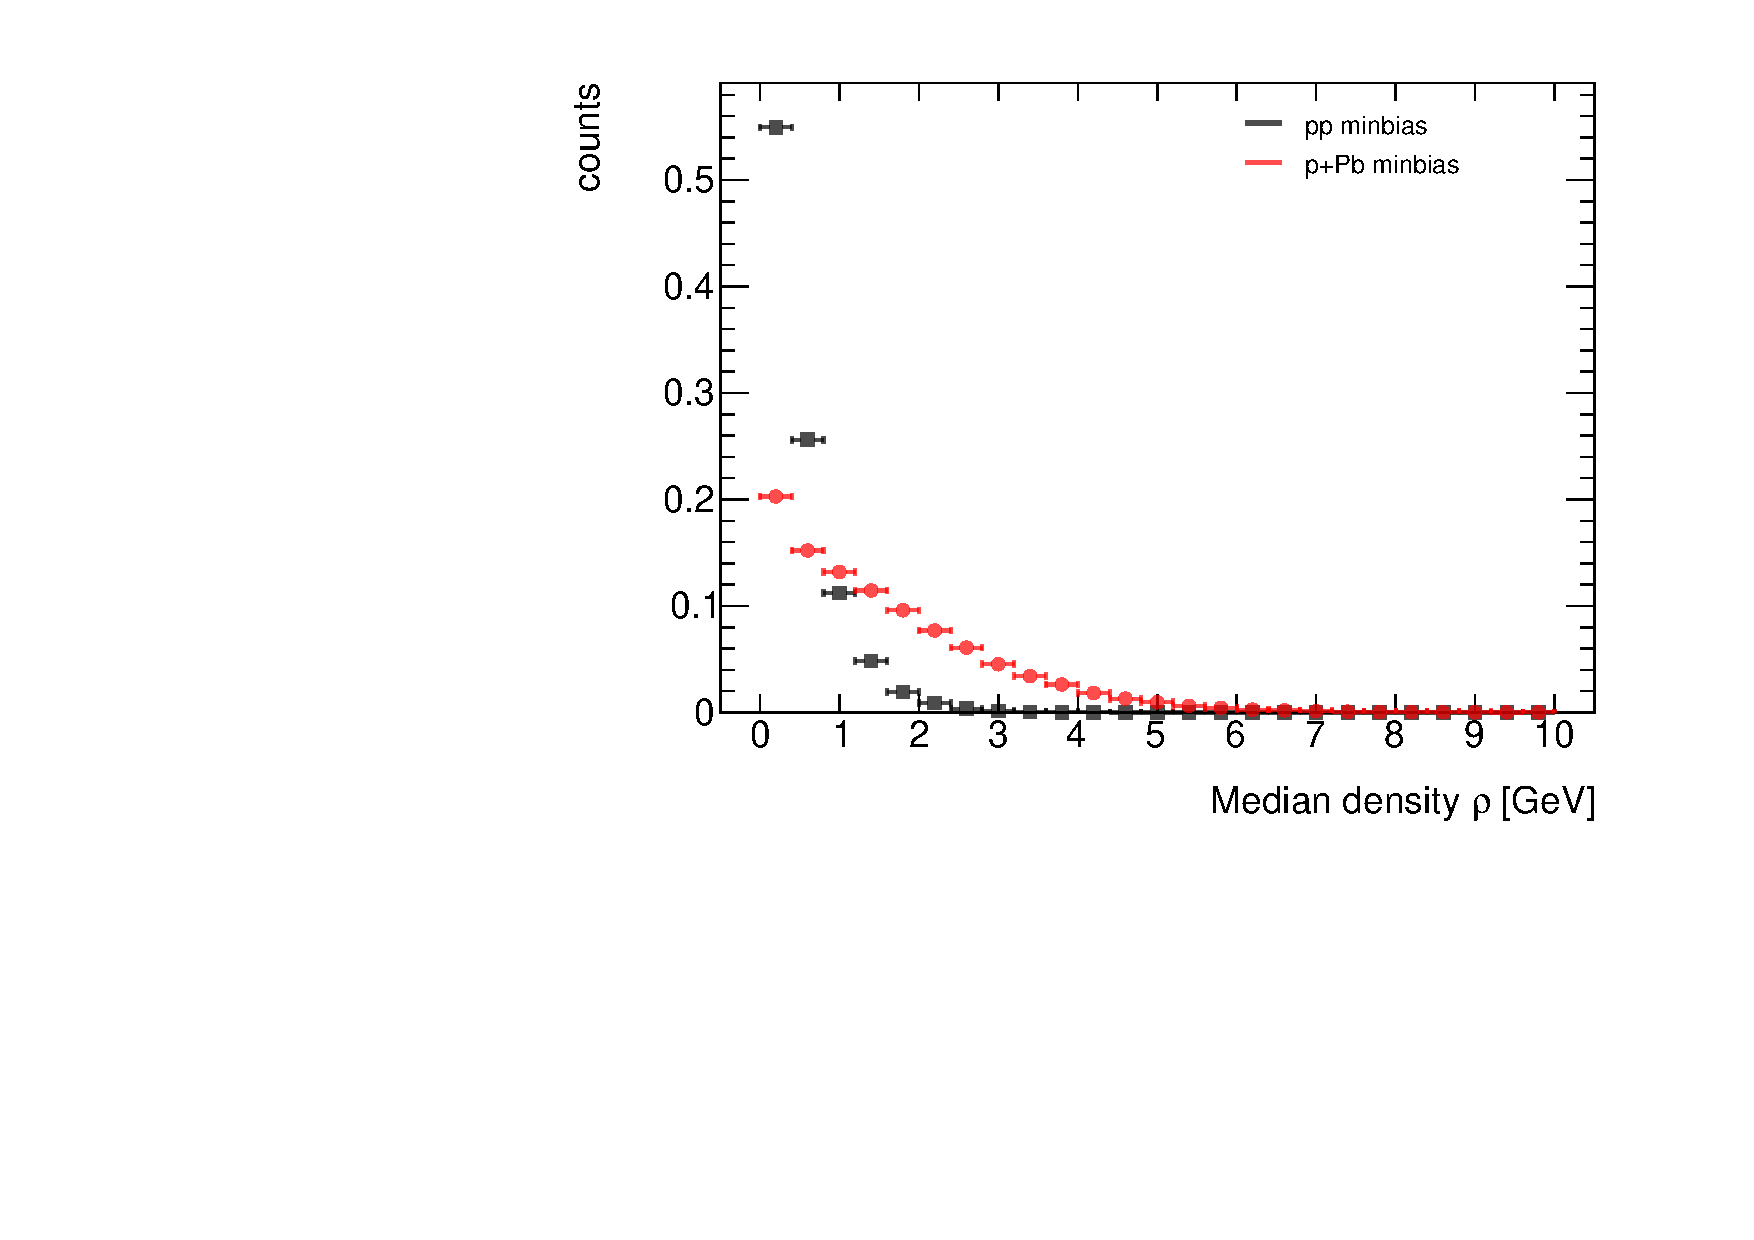
\includegraphics[width=0.49\textwidth]{UE/Rho_MinBias}
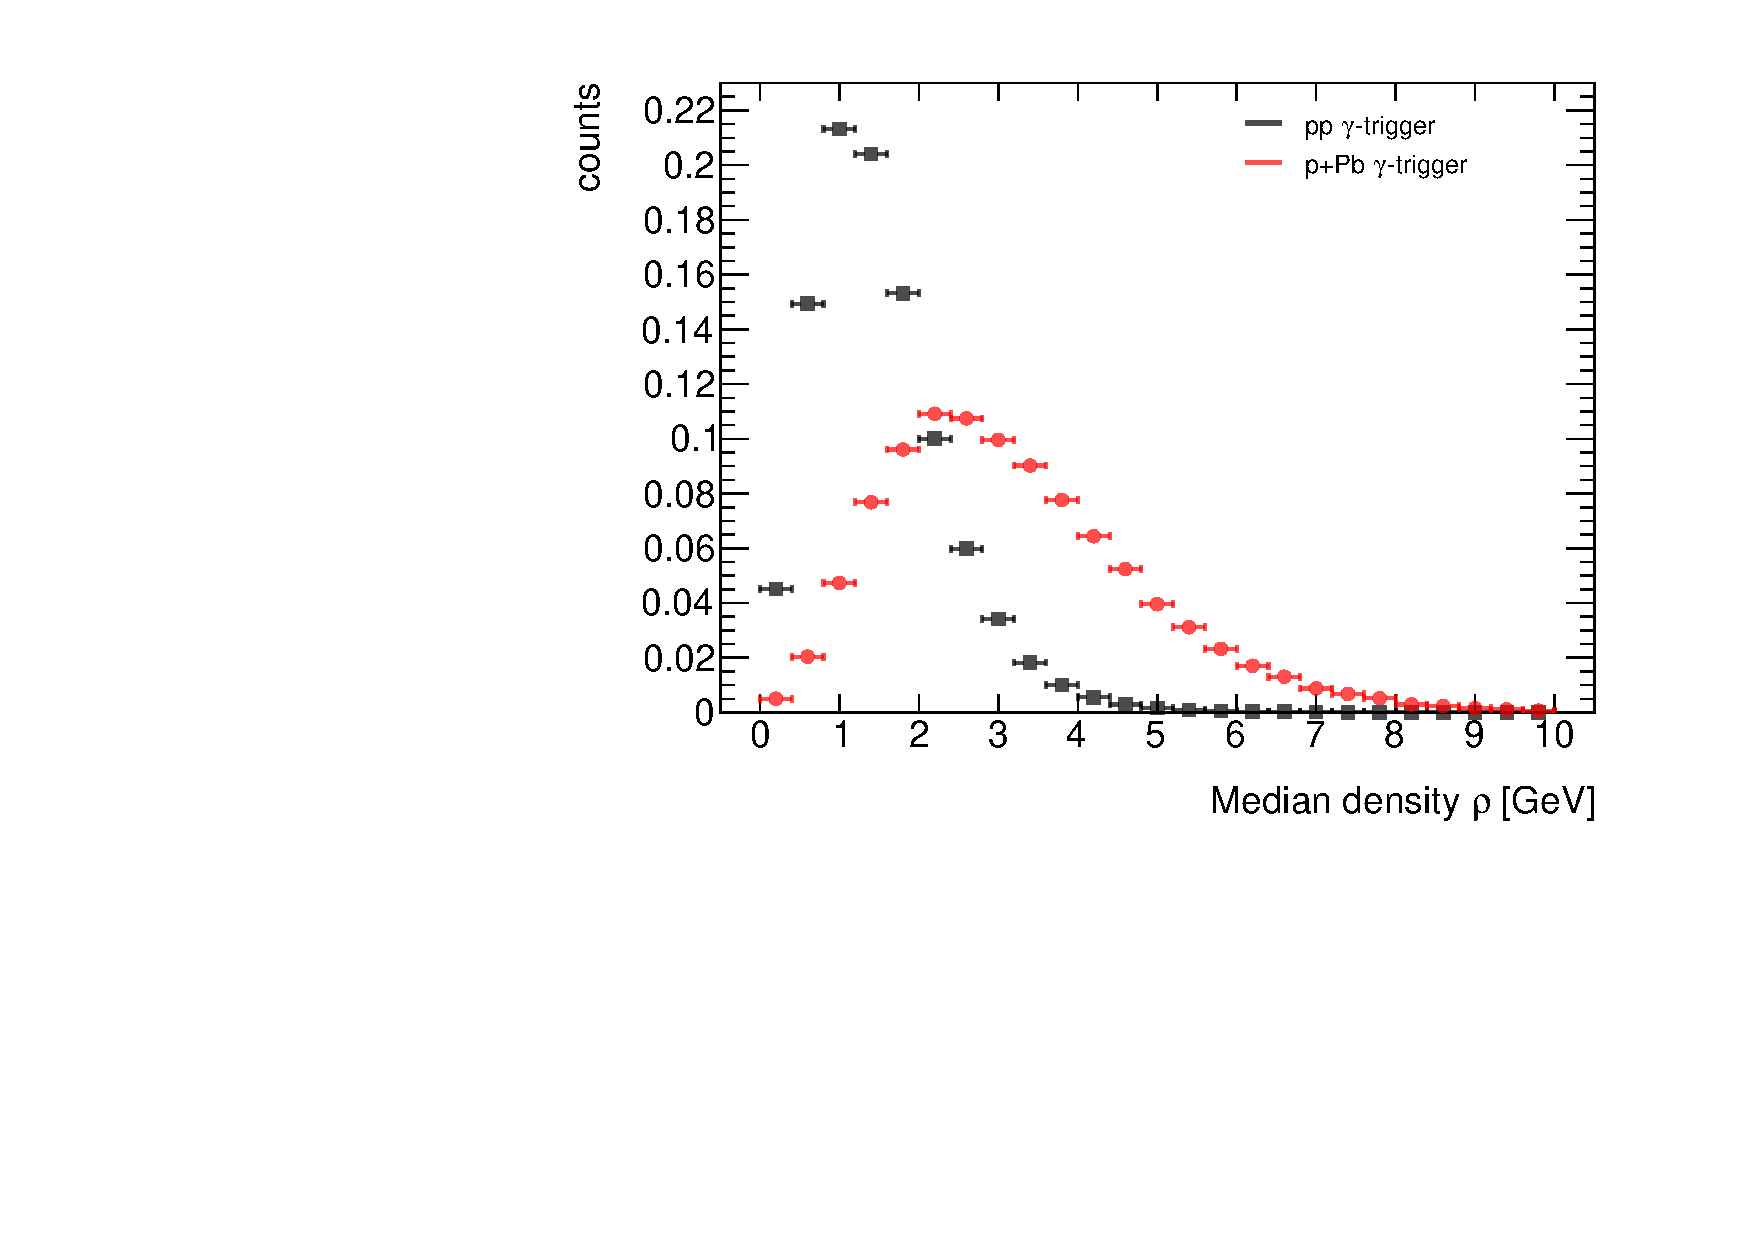
\includegraphics[width=0.49\textwidth]{UE/Rho_GammaTrigger}
\caption{Distribution of the median charged-particle transverse momentum density, $\rho$, in pp and \pPb~data, for a minimum-bias selection (left panel) and in photon-triggered events (right panel). }
\label{fig:Rho}
\end{figure}

The mean and standard deviation for each distribution is shown in Table~\ref{tab:rhoestimates}. The difference in UE-density in \pPb~is expected due to the increased number of nucleon-nucleon collisions. The UE-densities shown here are still about a factor of 50 lower than in central Pb-Pb collisions.
\begin{table}[h]
   \centering
   \caption{Median transverse momentum density mean and standard deviation in minimum-bias and and photon-triggered events in pp and \pPb~data. The statistical uncertainty in these numbers is negligible.}
   \label{tab:rhoestimates}
   \begin{tabular*}{1.0\columnwidth}{@{\extracolsep{\fill}}lcc|cc@{}}
    \hline
     &  pp minbias & pp $\gamma-$trigger & \pPb~ minbias & \pPb~$\gamma$-trigger  \\
       \hline
       $\langle\rho\rangle$   & 0.49 \GeVc & 1.51 \GeVc & 1.56 \GeVc & 3.19 \GeVc \\ 
       $\sigma_{\rho}$       &  0.47 \GeVc &  0.85 \GeVc  & 1.32 \GeVc & 1.60 \GeVc \\ 
            \hline        
   \end{tabular*}
\end{table}

The average $\rho$ for photon-triggered events reported in Table~\ref{tab:rhoestimates} is consistent with an independent estimate, based on the ``$\eta$-band'' method, that uses the same dataset and cluster selection~\cite{Erwann}. 


%\subsubsection{UE subtraction for jet transverse momentum}
%In this section, we show the result of using the measured median density to estimate UE-background for jets. We perform a jet-by-jet subtraction event-by-event. The subtracted transverse momentum of a given jet is:
%\begin{equation}
%  p_{\mathrm{T, rec}} = p_{\mathrm{T,raw}} - \rho \times A. 
%    \label{eq:jetsubtraction}
%\end{equation}
%\FloatBarrier
%Here $p_{\mathrm{T, rec}}$ is the raw transverse momentum and $A$ is the jet area.

%This approach neglects the fact that the UE-density for a given event is not uniform in $\eta$-$\phi$ but fluctuates from region to region. These fluctuations are mainly Poissonian but also encode correlated region-to-region variations of the particle multiplicity and mean $\pt$. 

%We check the impact of the fluctuations on the UE-subtraction by using Equation~\ref{eq:jetsubtraction} to measure the jet transverse momentum distribution in minimum-bias events, where the contribution from jets from a hard scattering is minimal and the reconstructed jets arise mainly from the UE and its fluctuations. That is, ideally the $p_{\mathrm{T, rec}}$ distribution should be a very narrow distribution centered around zero. 

%igure~\ref{fig:JetUE} shows the UE-subtracted transverse momentum distribution of jets in minimum-bias events in pp and p-Pb data. Only jets with $|\eta|<0.5$ are shown. In both cases, the distribution is centered around zero (the mean of the distribution if {$-$0.08 \GeVc} for pp and {0.02 \GeVc} for p-Pb data), and falls rather rapidly to both sides (the standard deviation is {1.13 \GeVc} for pp and {1.35 \GeVc} for p-Pb data). This demonstrates that the UE-subtraction for jet reconstruction works as intended. 

%\begin{figure}
%	\center
%	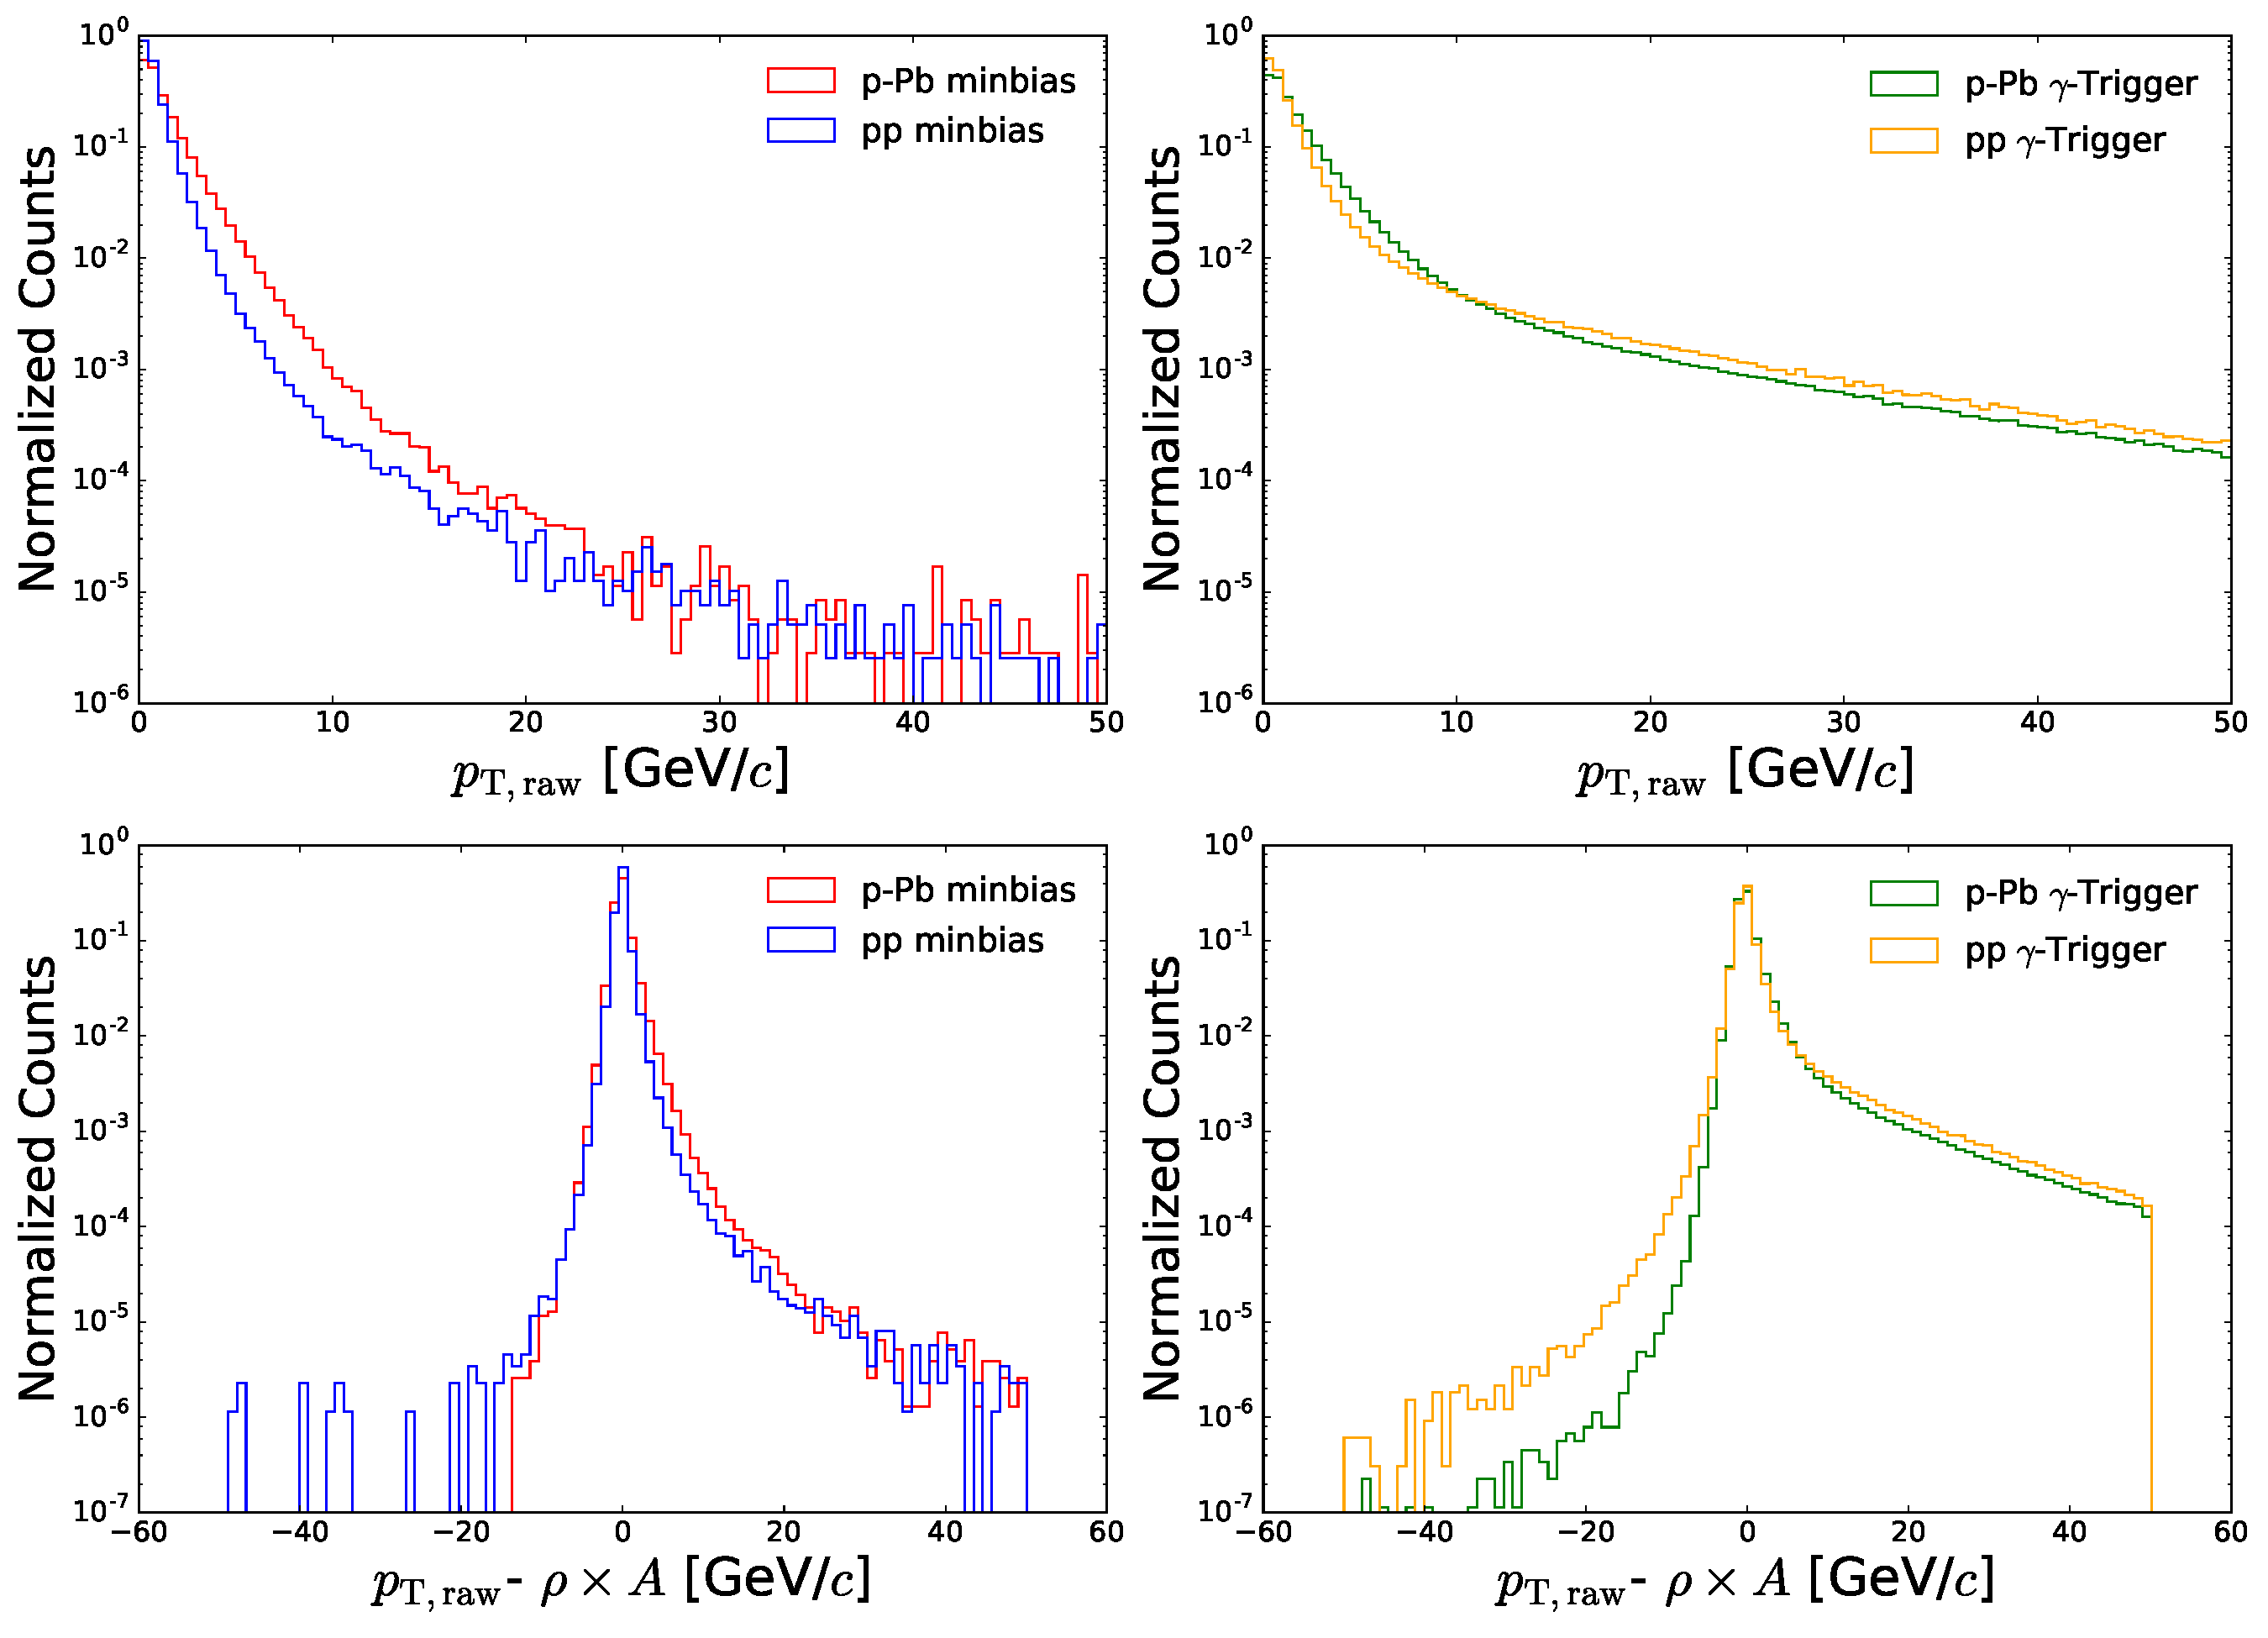
\includegraphics[width=0.9\textwidth]{UE/ppandpPb_jet_distributions.pdf}
%	\caption{A comparison between the jet transverse momentum distributions, both raw and  UE-subtracted, for minimum-bias and photon-triggered events in pp and p-Pb data. The raw jet transverse momentum distributions in minimum-bias events (upper left) and photon-triggered (upper right) in pp and p-Pb data are shown on the upper row. The UE-subtracted jet transverse momentum distributions in minimum-bias event (bottom left) and photon-triggered events (bottom right) in pp and p-Pb data are shown on the bottom row.}
%\label{fig:JetUE}
%\end{figure}

%The unphysical negative tail in Figure~\ref{fig:JetUE} arises due to UE over-subtraction. That is, the local UE density in the jet area is significantly lower than the calculated median density. On the other hand, the positive tail could be due to under-subtraction, however there are also a contribution from hard-scatterings in minimum-bias events, and there is a clear enhancement in photon-triggered events, as expected. 

%Table~\ref{TableUEUnderAndOverSubtraction} shows the fraction of jets shown in Figure~\ref{fig:JetUE} that satisfy a given threshold in subtracted  $p_{\mathrm{T, rec}}$. The results show that over-subtraction results in less than 0.5$\%$ of jets with $p_{\mathrm{T, rec}}<-3$ \GeVc. The fraction of jets with $p_{\mathrm{T, rec}}>5$ \GeVc~is less than a percent in minimum-bias p-Pb events, and drops to $0.13\%$ $p_{\mathrm{T, rec}}>10$ \GeVc. This informs our choice of minimum $p_{\mathrm{T, rec}}$ selection used for photon--jet analysis presented in Section~\ref{sec:GammaJet}. 

%\begin{table}[h]
%   \centering
%   \caption{Fraction of jets satisfying various UE-subtracted transverse momentum ranges in minimum bias events.}
%   \begin{tabular*}{1.0\columnwidth}{@{\extracolsep{\fill}}lccccc@{}}
%    \hline
%         &  pp minbias & p-Pb minbias  \\
%       \hline13

%       $p_{\mathrm{T,rec}}$ = $p_{\mathrm{T,raw}}$ - $\rho \times A$ $<$ $-$5.0 \GeVc & 0.05$\%$ & 0.05$\%$  \\ 
%       $p_{\mathrm{T,rec}}$ = $p_{\mathrm{T,raw}}$ - $\rho \times A$ $<$ $-$3.0 \GeVc & 0.32$\%$ & 0.46$\%$  \\
%       $p_{\mathrm{T,rec}}$ = $p_{\mathrm{T,raw}}$ - $\rho \times A$ $<$ $-$1.5 \GeVc & %3.24$\%$ & 5.28$\%$  \\
%       $p_{\mathrm{T,rec}}$ = $p_{\mathrm{T,raw}}$ - $\rho \times A$ $<\:\:\:\:\:\:\:\:\:\:\:$ 0 \GeVc & 63.52$\%$ & 61.55$\%$  \\
 %      \hline
 %      $p_{\mathrm{T,rec}}$ = $p_{\mathrm{T,raw}}$ - $\rho \times A$ $>\:\:\:$ 3.0 \GeVc & 1.02$\%$ & 2.73$\%$  \\
  %     $p_{\mathrm{T,rec}}$ = $p_{\mathrm{T,raw}}$ - $\rho \times A$ $>\:\:\:$ 5.0 \GeVc & 0.34$\%$ & 0.85$\%$  \\
 %      $p_{\mathrm{T,rec}}$ = $p_{\mathrm{T,raw}}$ - $\rho \times A$ $>\:\:\:$ 7.0 \GeVc & 0.16$\%$ & 0.34$\%$  \\
%       $p_{\mathrm{T,rec}}$ = $p_{\mathrm{T,raw}}$ - $\rho \times A$ $>$ 10.0 \GeVc & 0.08$\%$ & 0.13$\%$  \\
%    \hline
%%    \label{TableUEUnderAndOverSubtraction}
%	\end{tabular*}
%\end{table}

%Figure~\ref{fig:ppandpPb_mean_RhoA} shows the average UE energy that is subtracted on a jet-by-jet basis following Equation~\ref{eq:jetsubtraction}. There is a strong anti-correlation between the event $\rho$ and the jet area so while the density is a factor of 2 or so higher (as shown in Table~\ref{tab:rhoestimates}), the total average $\rho\times A$ is only about 20--30$\%$ higher in p-Pb collisions compared to pp collisions. 

%\begin{figure}[h]
%	\center
%	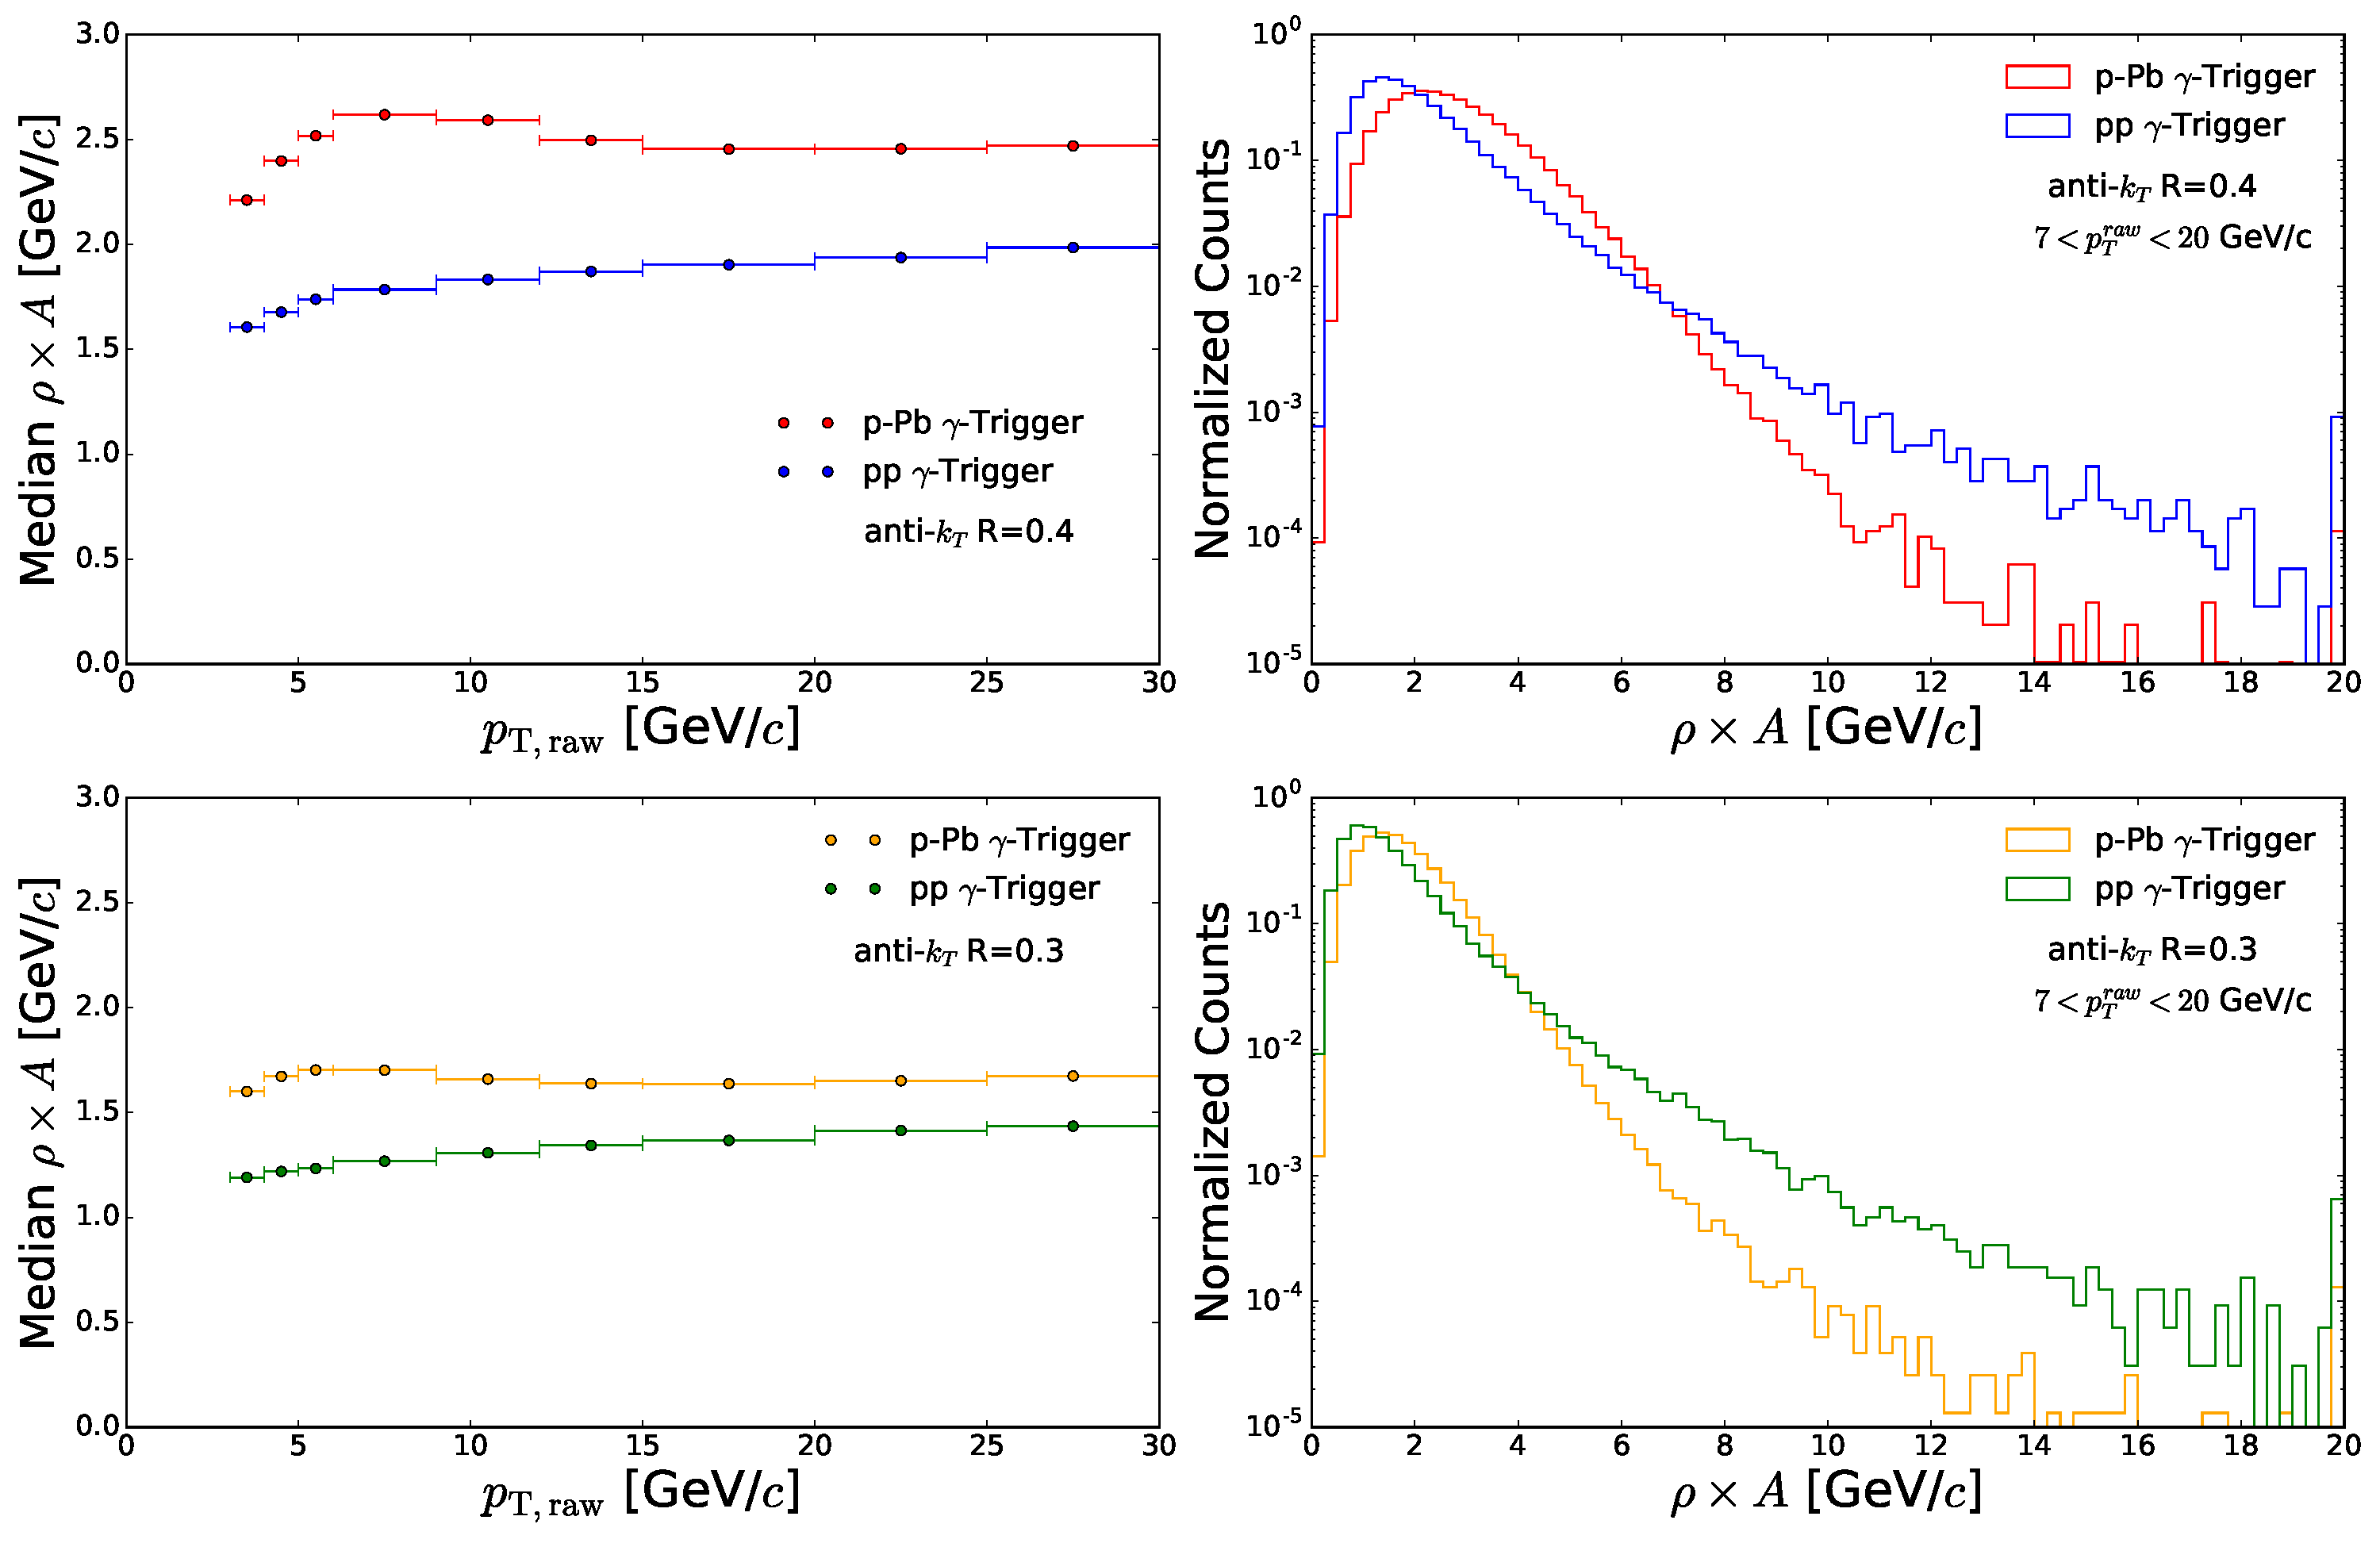
\includegraphics[width=0.99\textwidth]{JetReco/ppandpPb_median_AreaRho.pdf}
%	\caption{The average amount of UE-subtraction as a function of unsubtracted jet transverse momentum for photon-triggered events in pp and p-Pb data is shown on the left column for reconstructed jets of R = 0.3 and 0.4. The distribution of how much is UE-subtracted from jets with unsubtracted jet transverse momentum greater than {7 \GeVc} for photon-triggered events in pp and p-Pb data is shown on the right column for reconstructed jets of R = 0.3 and 0.4.}
%	\label{fig:ppandpPb_mean_RhoA}
%\end{figure}

%A recent study of of charged-jets cross-section at 7 TeV pp collisions~\cite{
%Acharya:2018eat} estimated that Multi Parton Interactions (MPIs) contribute about 50$\%$ of the cross-section for 5 $<\pt^{\mathrm{jet}}<$ 10 \GeVc~and about 20$\%$ for the range $\pt^{\mathrm{jet}}>$ 10 \GeVc. 

%This method requires the introduction of the jet area. According to the \textsc{FastJet} manual~\cite{Cacciari:2011ma}: \begin{quotation} {\it Jet areas provide a measure of the surface in the $y$-$\varphi$ plane over which a jet extends, or, equivalently, a measure of a jet’s susceptibility to soft contamination. Since a jet is made up of only a finite number of particles, one needs a specific definition in order to make its area an unambiguous concept.}\end{quotation} 

%The Voronoi~\footnote{The method used is the following fastjet::VoronoiAreaSpec \url{http://www.fastjet.fr/repo/doxygen-2.4.5/classfastjet_1_1VoronoiAreaSpec.html} }
%diagram associates each point in the $(\eta,
%\phi)$-plane with a unique track that is its nearest-neighbor by the
%Euclidean distance $\Delta R = \sqrt{\Delta\eta^2 + \Delta\phi^2}$.
%This particular choice (Euclidean Voronoi diagram) satisfies the conditions that:
%\begin{itemize}
%\item Each track resides inside the area associated with it;
%\item The sum over all areas associated with the tracks is unitary,
%  i.e.\ $3.6\pi$ for the ALICE tracking.
%\end{itemize}

%The boundary condition of the ALICE tracking at $\lvert\eta\rvert =
%0.9$ is treated as if no polygon may extend beyond, and is implemented
%using two ``mirror events'' where the particles are reflected by
%\begin{equation}
%  \eta \mapsto \pm 1.8 \mp \eta
%\end{equation}
%The cyclic boundary condition at $\lvert\phi\rvert = \pi$ is
%implemented by repeating the event with
%\begin{equation}
%  \phi \mapsto \phi \pm 2\pi
%\end{equation}
%(therefore nine copies of the same event occur during the construction
%of the Voronoi diagram).

%The empirical median function $\mathrm{med}$ is the Harrell--Davis quantile
%estimator $Q_p$ with $p =
%\frac{1}{2}$ (as opposed to the na\"{i}ve, inverse empirical
%cumulative distribution function method denoted $T_p$ therein). Note
%that unlike other definitions involving a truncated area forced to
%$\le \pi R^2$, the aforementioned properties of the Voronoi cells
%guarantee that all sparse areas are counted. This avoids the need of an ad-hoc correction factor, as used in Ref.~\cite{Adam:2015hoa}. Note that for the $k_{\mathrm{T}}$ algorithm, which is the one used for the UE estimation, the Voronoi area of a jet coincides with its ``passive area"~\cite{Cacciari:2011ma}, which is another standard \textsc{FastJet} method that has been used before by the ALICE Collaboration. 
